\documentclass[11pt,a4paper]{article}
\usepackage[utf8]{inputenc}
\usepackage[T1]{fontenc}
\usepackage[brazil]{babel}
\usepackage{geometry}
\usepackage{longtable}
\usepackage{booktabs}
\usepackage{array}
\usepackage{hyperref}
\usepackage{titlesec}
\usepackage{enumitem}
\usepackage{microtype}
\usepackage[htt]{hyphenat}
\usepackage{graphicx}
\usepackage{float}

\geometry{margin=1.8cm}
\hypersetup{colorlinks=true, linkcolor=black, urlcolor=blue}
\emergencystretch=3em
\sloppy

\newcolumntype{L}[1]{>{\raggedright\arraybackslash\small}p{#1}}
\setlength{\tabcolsep}{3pt}

\title{\textbf{Infraestrutura de Software}\\Implementação 1 --- ProcessFlow\\\large Relatório}
\author{Beatriz Loyola Gomes de Vasconcelos \\ \texttt{blgv@cesar.school}}
\date{24 de agosto de 2026}

\begin{document}
\maketitle

% NOTA: diretório e arquivo .tar de entrega devem se chamar blgv (blgv.tar),
% iniciais de blgv@cesar.school, conforme exigido no enunciado.

\section{Objetivo}

Este relatório documenta a implementação do \textbf{ProcessFlow}, um orquestrador de processos em C
capaz de cadastrar tarefas (\texttt{task}) e executá-las por meio de processos filhos criados com
\texttt{fork()}/\texttt{execvp()}. O programa suporta execução sequencial, paralela e em pipe entre
tarefas, redirecionamento de entrada/saída (\texttt{input}/\texttt{output}/\texttt{append}), troca de
diretório de trabalho (\texttt{workdir}), execução em background com controle de jobs
(\texttt{start}/\texttt{jobs}/\texttt{wait}) e dois modos de operação: interativo (prompt
\texttt{processflow>}) e workflow (leitura de um arquivo \texttt{.pf}). Todos os itens do enunciado
foram implementados e validados com os testes oficiais fornecidos pelo professor.

\section{Checklist de Requisitos}

\begin{longtable}{L{5.6cm} L{1.6cm} L{9.8cm}}
\toprule
\textbf{Requisito do enunciado} & \textbf{Status} & \textbf{Como testar / evidência} \\
\midrule
\endhead
Modo interativo com prompt \texttt{processflow>} & OK & Rodar \texttt{./processflow} sem argumentos \\
Modo workflow (\texttt{.pf}), ecoando cada linha antes de processar & OK & \texttt{./processflow teste.pf}; comparado via \texttt{diff} com \texttt{-saida.txt} esperado \\
Comando \texttt{exit} em ambos os modos & OK & Testado nas duas formas \\
Cadastro de tarefas (\texttt{task <nome> <programa> [args]}) & OK & \texttt{task listar /bin/ls -l} \\
\texttt{run sequential} & OK & \texttt{run sequential tarefa1 tarefa2 tarefa3} \\
\texttt{run parallel} & OK & Teste com \texttt{sleep 2}/\texttt{sleep 1} em paralelo, tempo total $\approx$2s \\
\texttt{run <tarefa>} sem palavra-chave (sequencial implícito) & OK & Exigido pelo \texttt{teste3} oficial; \texttt{args[1]} tratado como nome de tarefa quando não é keyword \\
Pipe entre tarefas (\texttt{run pipe}) & OK & \texttt{run pipe listar ordenar contar} $\to$ saída \texttt{13}, equivalente a \texttt{ls\textbar sort\textbar wc -l} \\
Redirecionamento (\texttt{input}/\texttt{output}/\texttt{append}) & OK & Teste com \texttt{sort}; \texttt{append} validado sem sobrescrever conteúdo prévio \\
\texttt{workdir <diretório>} & OK & \texttt{chdir()} com \texttt{perror} em caso de erro \\
Background (\texttt{start}), \texttt{jobs}, \texttt{wait <jobId>} & OK & \texttt{start processamento} imprime \texttt{[1] <PID>}; coleta de zumbis via \texttt{SIGCHLD} \\
Erros fatais (argc incorreto, workflow inexistente) & OK & Testado nos casos-limite (Fase 9) \\
Erros não fatais (tarefa/programa/arquivo/job/diretório inexistente) & OK & Programa segue processando após mensagem de erro \\
Linha vazia, múltiplos espaços, CTRL-D, workflow sem \texttt{exit} & OK & 5 casos-limite testados sem crash \\
Processos com exit code $\neq$ 0 e paralelos terminando fora de ordem & OK & Tratado sem interromper o orquestrador \\
\bottomrule
\end{longtable}

\section{Como Reproduzir}

\textbf{Compilar:}
\begin{verbatim}
make clean
make
\end{verbatim}

\textbf{Executar (modo interativo):}
\begin{verbatim}
./processflow
\end{verbatim}

\textbf{Executar (modo workflow):}
\begin{verbatim}
./processflow teste.pf
\end{verbatim}

\textbf{Exemplo de sessão:}
\begin{verbatim}
processflow> task listar /bin/ls -l
processflow> run sequential listar
processflow> task ordenar /usr/bin/sort
processflow> task contar /usr/bin/wc -l
processflow> run pipe listar ordenar contar
processflow> start listar
[1] 1234
processflow> jobs
processflow> wait 1
processflow> exit
\end{verbatim}

\section{Arquitetura (resumida)}

\textbf{Arquivos e responsabilidades:}
\begin{enumerate}[itemsep=2pt]
  \item \texttt{main.c} $\to$ loop principal (interativo e workflow), parsing de linha e dispatcher de comandos (\texttt{processar\_linha()}).
  \item \texttt{task.h}/\texttt{task.c} $\to$ struct \texttt{Task} e operações de cadastro/busca de tarefas, incluindo campos de redirecionamento.
  \item \texttt{exec.h}/\texttt{exec.c} $\to$ execução de processos: \texttt{spawn()} (fork+exec+wait), \texttt{spawn\_async()} (fork sem wait) e \texttt{run\_pipe()} (N-1 pipes encadeados).
  \item \texttt{job.h}/\texttt{job.c} $\to$ struct \texttt{Job} e gerência de jobs em background (criação, busca por PID, marcação de conclusão).
  \item \texttt{Makefile} $\to$ compilação (\texttt{all}), limpeza (\texttt{clean}), flags \texttt{-Wall -Wextra}.
\end{enumerate}

\textbf{Decisões técnicas:}
\begin{enumerate}[itemsep=2pt]
  \item \textbf{Array fixo (\texttt{char *args[64]}) em vez de lista encadeada} $\to$ \texttt{execvp} exige vetor contíguo terminado em \texttt{NULL} $\to$ simplifica o parsing, ao custo de um limite fixo de argumentos.
  \item \textbf{Separação em módulos} (\texttt{task}, \texttt{exec}, \texttt{job}) em vez de tudo em \texttt{main.c} $\to$ isola dados de execução $\to$ facilita manutenção e reuso (ex.: \texttt{spawn\_async()} reaproveitado tanto por \texttt{run parallel} quanto por \texttt{start}).
  \item \textbf{\texttt{Task} vs. \texttt{Job} como entidades distintas} $\to$ \texttt{Task} é definição estática reutilizável, \texttt{Job} é uma execução específica com identidade própria (job\_id, PID, status) $\to$ permite múltiplas execuções em background da mesma tarefa sem conflito.
  \item \textbf{Coleta de zumbis via handler de \texttt{SIGCHLD}} (\texttt{waitpid(-1, \&status, WNOHANG)} em loop) em vez de depender só de \texttt{wait} manual $\to$ jobs terminados saem da lista automaticamente $\to$ evita acúmulo de processos zumbis.
\end{enumerate}

\section{Estratégias e Diário de Desenvolvimento}

\subsection{Estratégias da semana}

\begin{longtable}{L{1.2cm} L{3.5cm} L{7.5cm} L{4.7cm}}
\toprule
\textbf{Estrat.} & \textbf{Nome curto} & \textbf{Contexto} & \textbf{Motivo da troca} \\
\midrule
\endhead
S1 & Parser + dispatcher em array fixo & Tokenização de linha com \texttt{strtok}, despacho via \texttt{strcmp} em cadeia \texttt{if/else if}. Array fixo (\texttt{char *args[64]}) escolhido por \texttt{execvp} exigir vetor contíguo terminado em \texttt{NULL}. & --- \\
S2 & Módulos separados (\texttt{task}/\texttt{exec}) & Separação de responsabilidades: \texttt{task.c} cuida de dados, \texttt{exec.c} cuida de fork/exec/wait. & --- \\
S3 & Pipe com N-1 pipes + \texttt{dup2} encadeado & \texttt{run\_pipe()} cria todos os pipes antes de qualquer fork; cada filho faz \texttt{dup2} conforme posição na cadeia e fecha todos os fds antes do exec. & --- \\
S4 & Redirecionamento via campos na struct \texttt{Task} & Campos \texttt{input\_file}/\texttt{output\_file}/\texttt{append\_file}; \texttt{spawn()} abre o arquivo e faz \texttt{dup2} antes do \texttt{execvp}. & --- \\
S5 & Dispatcher extraído para \texttt{processar\_linha()} & Refatorado para reaproveitar o mesmo parser entre modo interativo e modo workflow. & --- \\
S6 & Módulo \texttt{job.h}/\texttt{job.c} & Struct \texttt{Job} (job\_id, pid, nome\_task, status) espelhando o padrão de \texttt{task.c}. & --- \\
S7 & Background via \texttt{spawn\_async()} + \texttt{SIGCHLD} & \texttt{start} reaproveita \texttt{spawn\_async()}; zumbis coletados por handler de \texttt{SIGCHLD}. & --- \\
\bottomrule
\end{longtable}

\subsection{Diário de Tentativas}

\begin{longtable}{L{0.5cm} L{1.1cm} L{4.5cm} L{2.7cm} L{7.5cm}}
\toprule
\textbf{\#} & \textbf{Estrat.} & \textbf{O que tentei} & \textbf{Resultado} & \textbf{Hipótese/\allowbreak Causa (se falhou)} \\
\midrule
\endhead
1 & S1 & Loop interativo com \texttt{fgets} + prompt \texttt{processflow>} & OK & --- \\
2 & S1 & Tokenização com \texttt{strtok}, guardando ponteiros em \texttt{args[64]} & Falha parcial $\to$ corrigida & \texttt{strcpy(args[i], token)} em ponteiro não inicializado; corrigido para atribuição direta do ponteiro. \\
3 & S2 & Struct \texttt{Task} com \texttt{char *argumentos[64]} & Falha parcial $\to$ corrigida & Array de tamanho flexível na struct sem alocação manual; trocado para tamanho fixo. \\
4 & S2 & \texttt{criar\_task()} copiando dados para a struct & Falha parcial $\to$ corrigida & \texttt{strcpy} em ponteiros não alocados (trocado por \texttt{strdup}); índice sempre 0 por uso de \texttt{->} em array (corrigido para indexação explícita). \\
5 & S2 & \texttt{encontrar\_task()} por nome & Falha parcial $\to$ corrigida & \texttt{strcmp} comparando string com struct; retorno por valor em função que devia retornar \texttt{Task*}. \\
6 & S2 & \texttt{spawn()}: fork+execvp+waitpid & Falha parcial $\to$ corrigida & Faltava \texttt{exit(1)} no filho após \texttt{execvp} falhar, duplicando o loop do pai. \\
7 & S1/S2 & Teste ponta a ponta: \texttt{task listar} + \texttt{run sequential} & OK & --- \\
8 & S2 & Testes de erro (tarefa/programa inexistente, args insuficientes) & OK & --- \\
9 & S2 & Makefile (\texttt{all}/\texttt{clean}, \texttt{-Wall -Wextra}) & OK & --- \\
10 & S1 & \texttt{run sequential} generalizado para N tarefas & Falha parcial $\to$ corrigida & Loop usava \texttt{args[2]} fixo em vez de \texttt{args[i]}. \\
11 & S2 & \texttt{run parallel} via \texttt{spawn\_async()} & Falha parcial $\to$ corrigida & \texttt{return;} em função \texttt{pid\_t} sem valor; \texttt{waitpid} chamado com \texttt{pids[i]==-1} bagunçando espera de outros filhos. \\
12 & S2 & Paralelismo real (\texttt{sleep 2}/\texttt{sleep 1}) & OK & --- \\
13 & S3 & Primeira versão de \texttt{run\_pipe()} & Falha parcial $\to$ corrigida & \texttt{if (pids[i == 0])} com parênteses trocados; \texttt{else if} impedia os dois \texttt{dup2} nos processos do meio. \\
14 & S3/S5 & Teste \texttt{run pipe listar ordenar contar} + ligação no dispatcher & OK & --- \\
15 & S4 & Campos \texttt{input\_file}/\texttt{output\_file}/\texttt{append\_file} + comandos & Falha parcial $\to$ corrigida & Checagem errada de \texttt{args[1]} em vez de \texttt{args[0]}, com loop desnecessário; reescrito sem loop. \\
16 & S4 & \texttt{spawn()}: \texttt{open()} + \texttt{dup2} antes do \texttt{execvp} & OK & --- \\
17 & S4 & Teste \texttt{input}/\texttt{output}/\texttt{append} & OK & --- \\
18 & S5 & Extração para \texttt{processar\_linha()} & Falha parcial $\to$ corrigida & \texttt{continue} de loops internos (sequential/parallel) virou \texttt{return}, abortando a função inteira; revertido. \\
19 & --- & Chaves desbalanceadas em \texttt{main.c} & Falha $\to$ corrigida & Faltava fechar \texttt{main}; depois \texttt{return 0;} preso dentro do \texttt{while(1)}. \\
20 & S5 & Modo workflow (\texttt{argc==2}) & OK (após recompilar) & --- \\
21 & S5 & \texttt{workdir <dir>} com \texttt{chdir()} & OK & --- \\
22 & S6 & \texttt{criar\_job()} em \texttt{job.c} & Falha parcial $\to$ corrigida & Incremento do contador antes de usar como índice causava overflow do array. \\
23 & S6 & Retorno do \texttt{job\_id} criado & Falha parcial $\to$ corrigida & Leitura após incrementar contador, apontando para slot não inicializado. \\
24 & S6 & \texttt{marcar\_job\_concluido(pid\_t pid)} & Falha parcial $\to$ corrigida & Reaproveitou busca por \texttt{job\_id} passando \texttt{pid}; corrigido com busca dedicada por \texttt{pid}. \\
25 & S6 & \texttt{listar\_jobs()} antiga & Código morto removido & \texttt{status\_str} não inicializado seguido de \texttt{strcpy}. \\
26 & S7 & Ligação \texttt{start}/\texttt{jobs}/\texttt{wait} no dispatcher & Falha parcial $\to$ corrigida & \texttt{strcmp(args[0], "jobs")} sem \texttt{==0}. \\
27 & S7 & Teste \texttt{start} com programa inexistente & Comportamento correto & Job criado no \texttt{fork()} antes de saber se \texttt{execvp} funciona --- assíncrono, esperado. \\
28 & S7 & \texttt{sigchld\_handler()} com \texttt{waitpid(-1,\&status,WNOHANG)} & OK & --- \\
29 & --- & Revisão de erros: \texttt{run\_pipe()} sem aviso de falha de \texttt{fork()} & Falha parcial $\to$ corrigida & \texttt{return;} no meio do loop abandonava filhos já criados; corrigido para só avisar e seguir. \\
30 & --- & Casos-limite: linha vazia, espaços múltiplos, CTRL-D, workflow sem \texttt{exit}, args inválidos, exit code $\neq$0 & OK & --- \\
31 & --- & Testes oficiais \texttt{teste1}/\texttt{teste2}/\texttt{teste3} & Falha $\to$ corrigida & \texttt{teste3} usa \texttt{run escrever} sem keyword; dispatcher exigia \texttt{argc\_line>=3}. Corrigido com caso implícito (sequencial por padrão). \\
32 & --- & \texttt{diff} da saída do \texttt{teste3} vs. esperado & Falha parcial $\to$ corrigida & \texttt{stdout} do pai fully-buffered ao redirecionar para arquivo, saída dos filhos saía antes do eco das linhas; corrigido com \texttt{fflush(stdout)} após cada \texttt{printf} de eco. \\
33 & --- & Comparação de \texttt{teste1}/\texttt{teste2} & Falha aparente, não era bug & Esses testes usam \texttt{stdin} redirecionado (modo interativo), não \texttt{.pf}; validado com \texttt{./processflow < entrada.txt}, saída bateu 100\%. \\
\bottomrule
\end{longtable}

\textit{Nota: as colunas "Quando" e "Evidência" foram omitidas da tabela --- todas as tentativas têm como evidência o arquivo \texttt{evidencias.log} (gerado com \texttt{script -a evidencias.log}), que
registra em ordem cronológica os comandos e saídas de toda a sessão de desenvolvimento.}

\section{Evidências}

O arquivo \texttt{evidencias.log} (gerado via \texttt{script -a evidencias.log}) registra integralmente os
comandos e saídas de todas as sessões de trabalho (19/08 e 23/08), incluindo \texttt{date}, \texttt{whoami}
e \texttt{pwd} no início de cada sessão, e é enviado junto com o código-fonte no \texttt{.tar}. Os principais
pontos de evidência:

\begin{itemize}[itemsep=2pt]
  \item \textbf{Erro principal da semana}: bug de \texttt{dup2} nos processos do meio do pipe (tentativa 13), que impedia a leitura e escrita simultâneas por causa de um \texttt{else if} incorreto.
  \item \textbf{Validação final}: execução dos três testes oficiais do professor (\texttt{teste1}, \texttt{teste2}, \texttt{teste3}) com \texttt{diff} limpo contra as saídas esperadas (tentativas 31--33).
  \item \textbf{Achado de buffering}: diferença de comportamento de \texttt{stdout} entre terminal (line-buffered) e saída redirecionada para arquivo (fully buffered), só percebida ao testar com \texttt{> arquivo} (tentativa 32).
\end{itemize}

\subsection{Prints}

\begin{figure}[H]
  \centering
  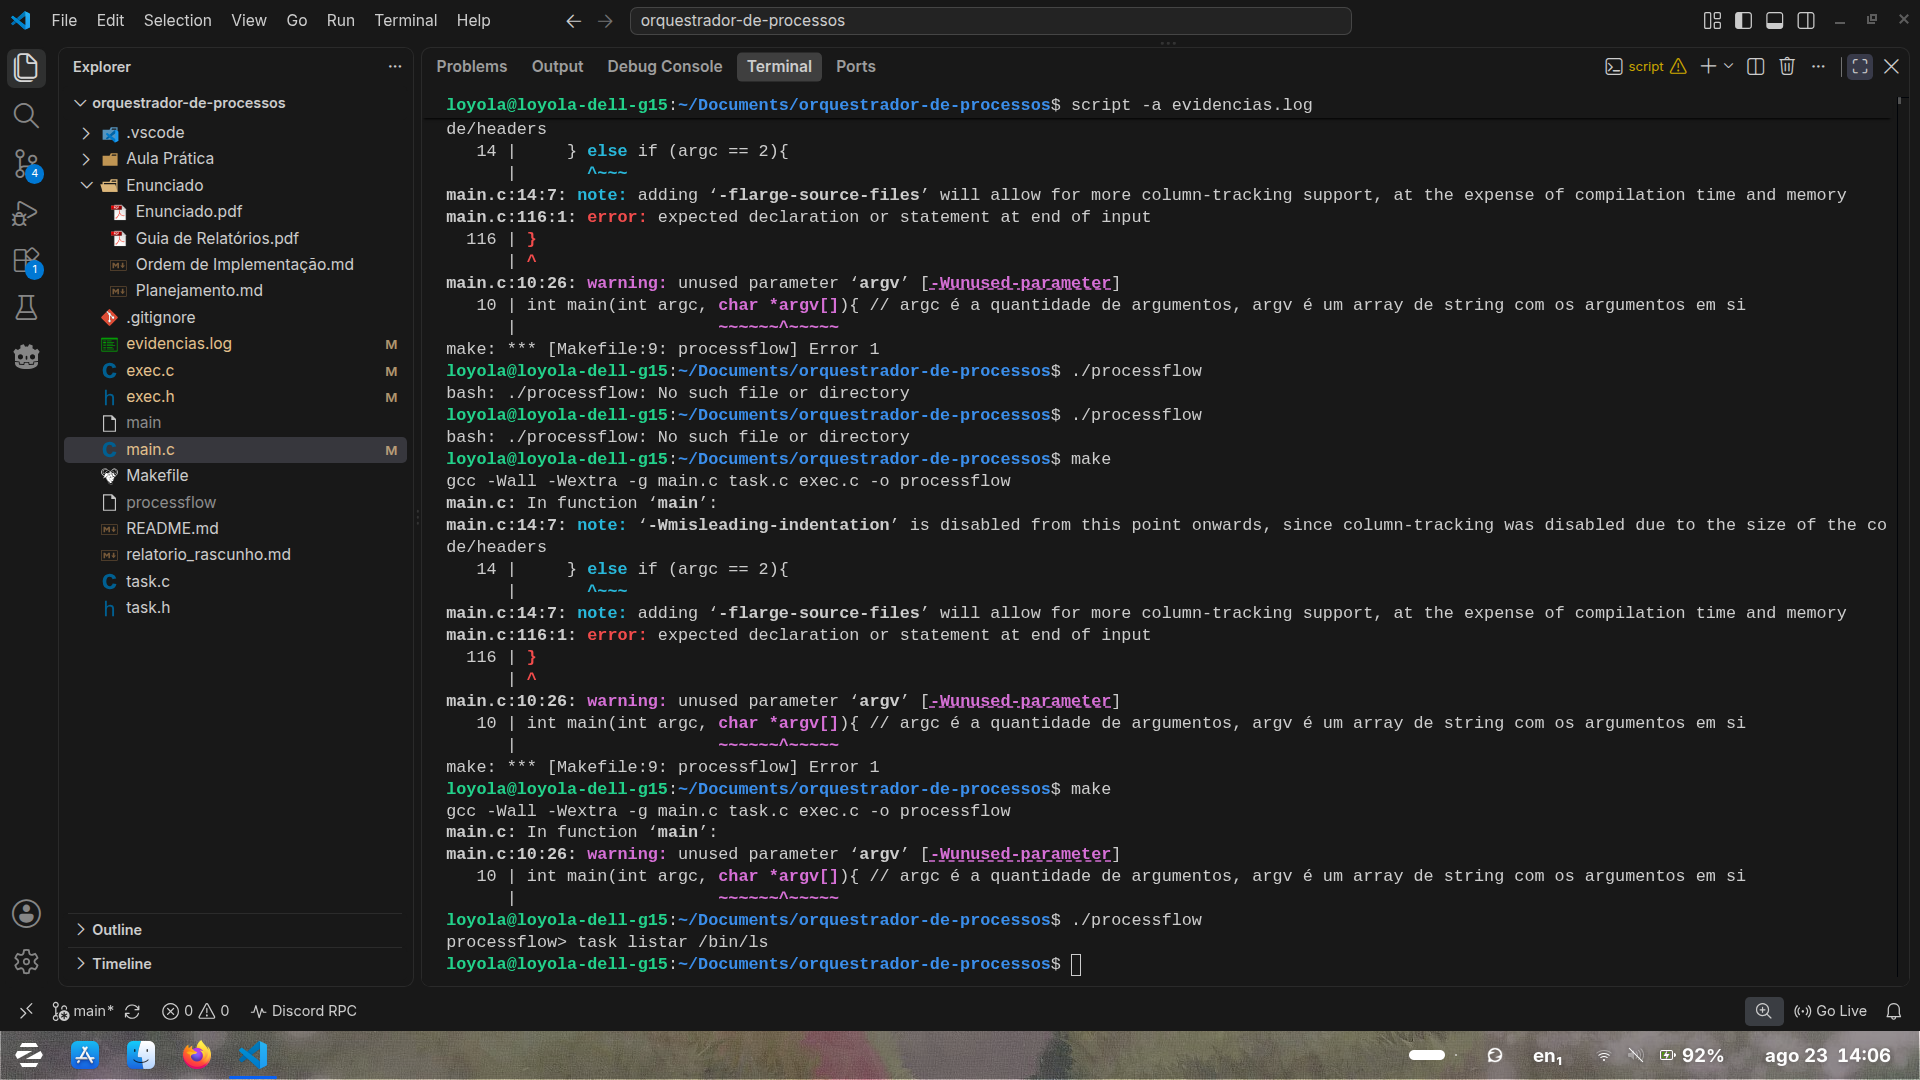
\includegraphics[width=0.92\textwidth]{Prints/erro-principal.png}
  \caption{Erro principal da semana: chaves desbalanceadas em \texttt{main.c} após edições manuais
  (\texttt{main.c:116:1: error: expected declaration or statement at end of input}, tentativa \#19),
  seguido da correção e recompilação bem-sucedida.}
\end{figure}

\begin{figure}[H]
  \centering
  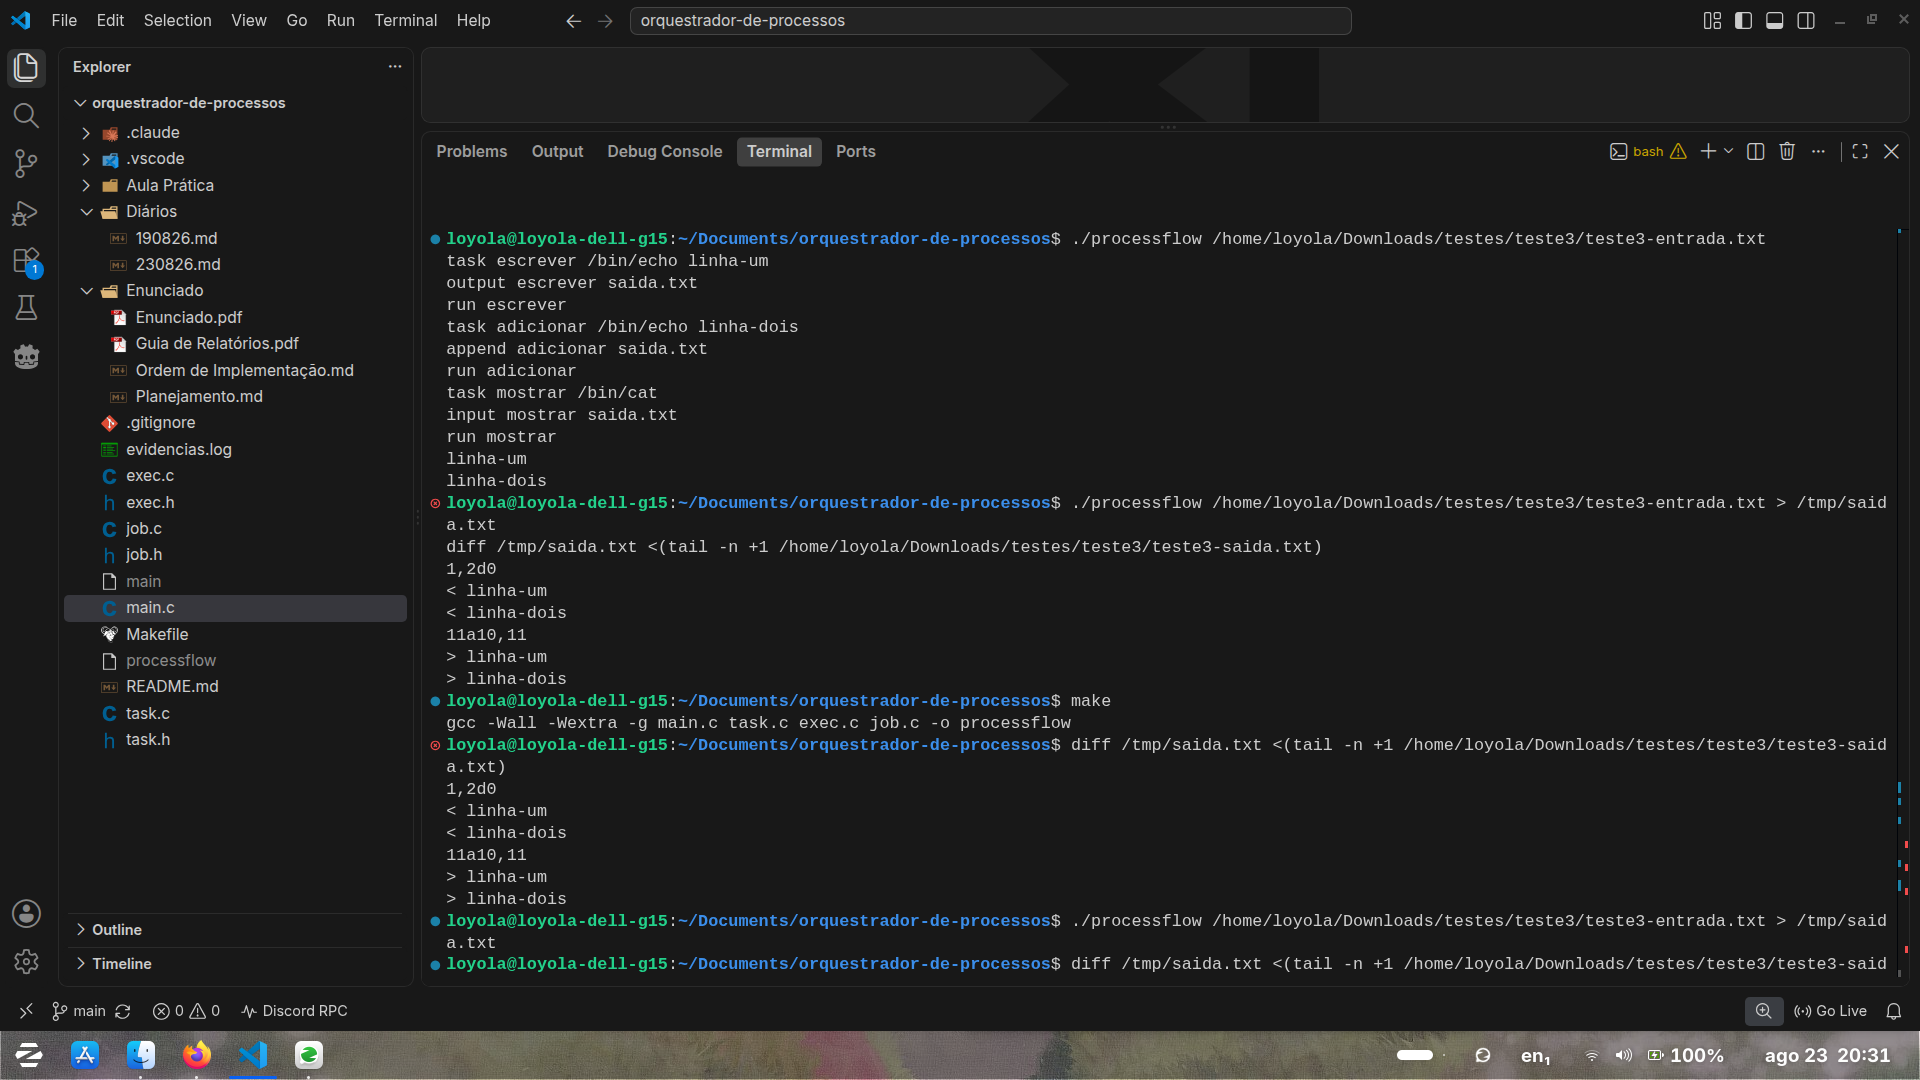
\includegraphics[width=0.92\textwidth]{Prints/validacao-final.png}
  \caption{Validação final: \texttt{diff} entre a saída do \texttt{teste3} oficial e o resultado esperado,
  limpo após a correção do \texttt{fflush(stdout)} no eco de linhas do modo workflow (tentativas \#31--32).}
\end{figure}

\begin{figure}[H]
  \centering
  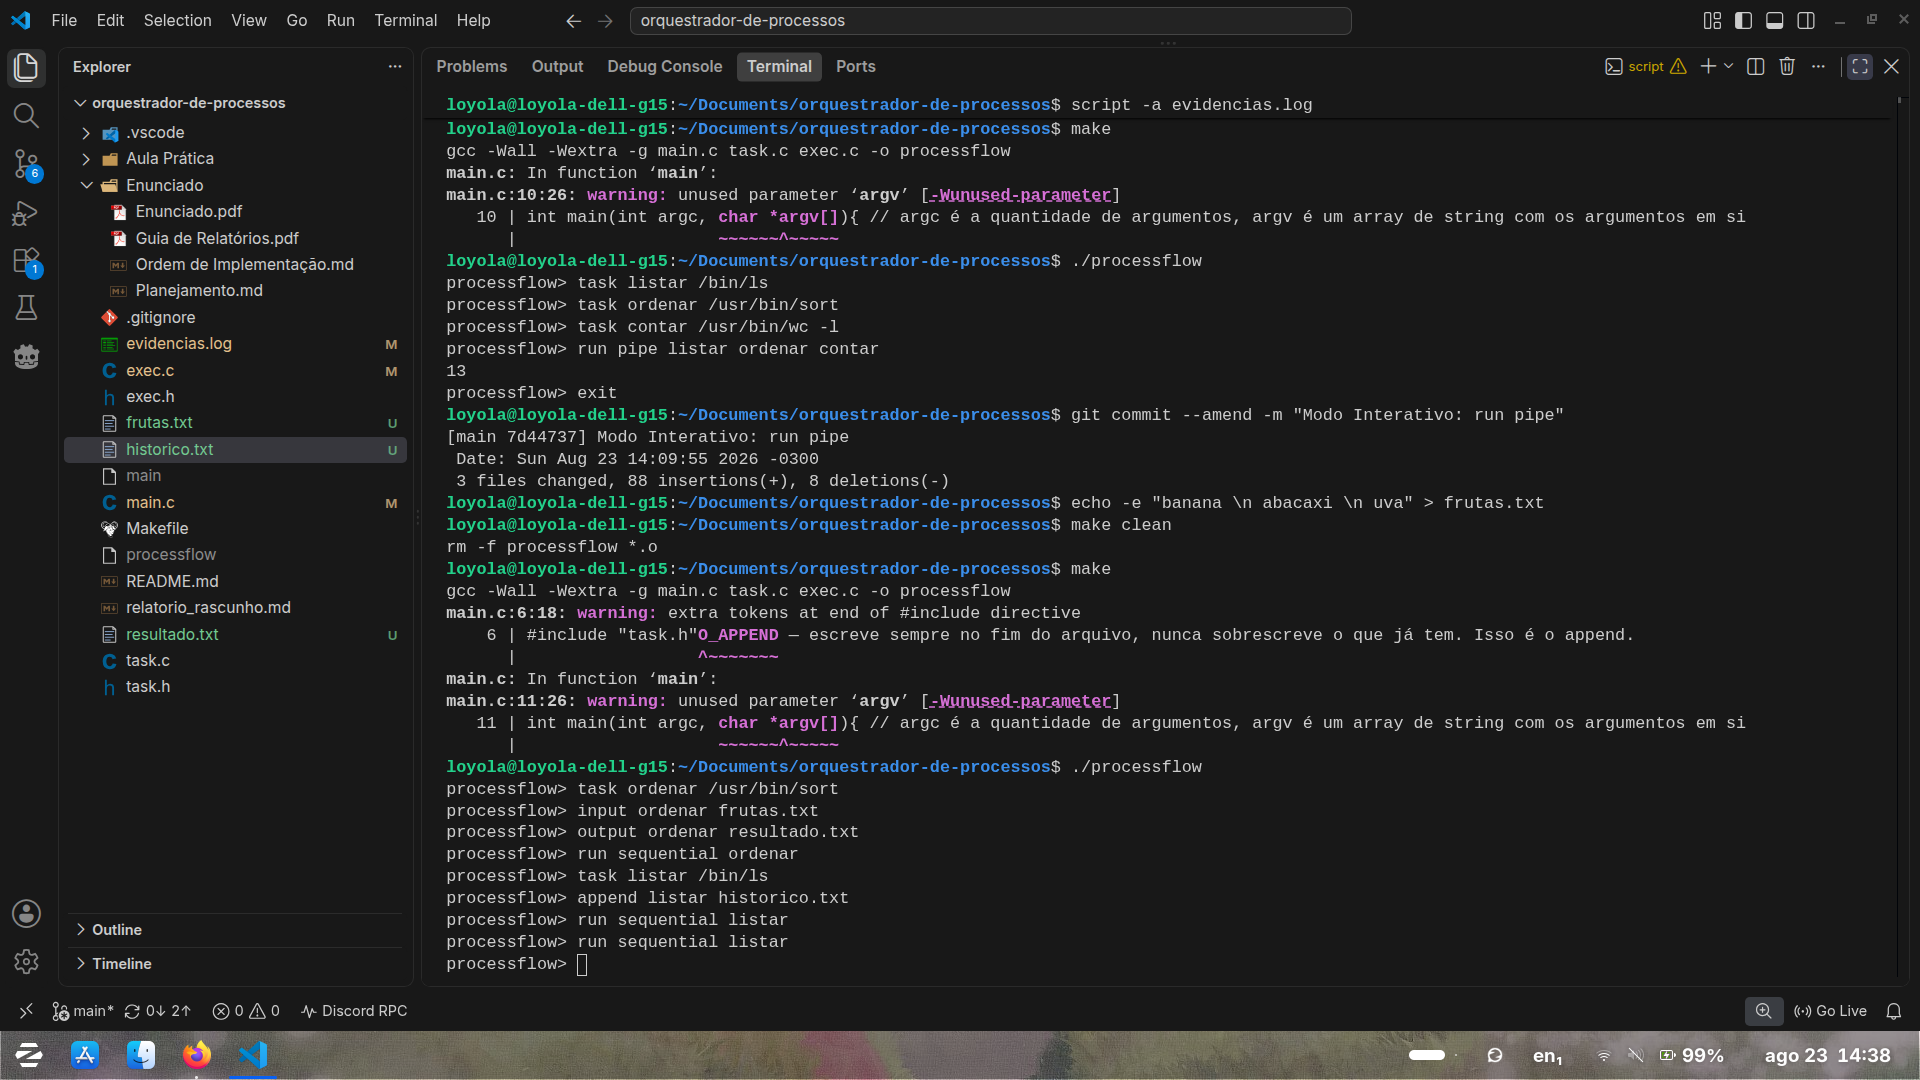
\includegraphics[width=0.92\textwidth]{Prints/pipe-redirecionamento.png}
  \caption{Teste ponta a ponta de \texttt{run pipe listar ordenar contar} (saída \texttt{13}) e de
  redirecionamento (\texttt{input}/\texttt{output}/\texttt{append}), confirmando pipe e redirecionamento
  funcionando em conjunto.}
\end{figure}

\section{Uso de IA}

\textbf{Onde usei IA:} utilizada como mentora/revisora de código durante todo o desenvolvimento --- não
escreveu a lógica principal do programa, mas apontou bugs (ponteiros não inicializados, tipos incompatíveis
entre struct e string, erros de escopo em refatoração), explicou conceitos de C (\texttt{strtok},
\texttt{fork}/\texttt{exec}/\texttt{wait}, \texttt{dup2}, \texttt{SIGCHLD}) e ajudou a montar o Makefile.

\textbf{Prompts principais:} pedidos de revisão de trechos de código com bug suspeito; explicações sobre
manipulação de descritores de arquivo e pipes; dúvidas conceituais sobre diferença entre buffering de
terminal e de arquivo.

\textbf{O que validei manualmente:} cada trecho corrigido foi testado rodando \texttt{./processflow} com
casos reais (tarefas de teste, pipes, redirecionamento, background) antes de prosseguir para a próxima
etapa; todos os testes oficiais do professor foram validados com \texttt{diff} contra as saídas esperadas.

\section{Reflexão Final}

O desenvolvimento revelou dois padrões de bug recorrentes que se repetiram em módulos diferentes: (1)
ponteiros não inicializados usados com \texttt{strcpy} em vez de alocação com \texttt{strdup}, e tipos
incompatíveis entre struct e string em comparações/retornos; (2) inversão da ordem "usar índice, depois
incrementar" vs. "incrementar, depois usar índice", que apareceu tanto em \texttt{criar\_task} quanto em
\texttt{criar\_job}. Isso indica que, com mais tempo, valeria a pena extrair um padrão utilitário comum para
criação de entidades em arrays estáticos (tasks/jobs), reduzindo a chance de repetir o mesmo erro. A
separação em módulos (\texttt{task}, \texttt{exec}, \texttt{job}) e a extração do dispatcher em
\texttt{processar\_linha()} foram decisões acertadas, pois permitiram reaproveitar a mesma lógica entre modo
interativo e workflow, e reaproveitar \texttt{spawn\_async()} entre \texttt{run parallel} e \texttt{start}.
O bug mais custoso foi o de buffering de \texttt{stdout} ao redirecionar a saída para arquivo, só descoberto
ao comparar a saída do \texttt{teste3} via \texttt{diff} --- lição de que testes manuais no terminal não são
suficientes e é preciso sempre testar também com saída redirecionada.

\section{Checklist Final de Entrega}

\begin{longtable}{L{11cm} L{3cm}}
\toprule
\textbf{Item} & \textbf{Confirmado?} \\
\midrule
\endhead
Compilei do zero seguindo só o que está no relatório & Sim \\
Rodei os testes e \texttt{evidencias.log} foi gerado & Sim \\
Tenho prints obrigatórios & Sim \\
Testei pelo menos um caso limite e um caso inválido & Sim \\
Preenchi a seção de uso de IA & Sim \\
Revisei o relatório e removi frases genéricas / vazias & Sim \\
\bottomrule
\end{longtable}

\section{Se eu tivesse mais 2 horas}

Investiria em: (1) tratamento mais robusto de limites fixos (\texttt{args[64]}, \texttt{tasks[64]},
\texttt{jobs[64]}), avisando o usuário ao invés de falhar silenciosamente ao estourar; (2) organização do
\texttt{evidencias.log} em seções por sessão para facilitar a leitura cruzada com a tabela de tentativas.

\end{document}
